%% Standalone lecture -- build with:  pdflatex -shell-escape eigensystems
%% Shared preamble for standalone lecture files.
%%
%% Every lecture begins with %% Shared preamble for standalone lecture files.
%%
%% Every lecture begins with %% Shared preamble for standalone lecture files.
%%
%% Every lecture begins with \input{preamble} and is compiled on its own:
%%     pdflatex -shell-escape <lecture>
%% There is no master lectures.tex any more -- the list of lectures lives in
%% lectures.yaml and is read by the build scripts.

\documentclass[25pt,landscape,footrule]{foils}
\input{macros_gen}
\backgroundsetup{contents={}}

\usepackage{stmaryrd}
\usepackage{ifthen}
\usepackage{pdf14}

% Every figure lives in this course's lectures/figures (consolidated
% 2026-10-08).  Do not add other courses' folders back: when a name exists in
% several folders LaTeX silently takes the first, which mixed old and new
% frames of the same animation.  A missing figure should be a build error.
\graphicspath{{figures/}{../lectures/figures/}}

\date{}

\newcounter{lessoncnt}
\newcommand{\lesson}[1]{\setcounter{page}{1}%
\section{Mathematics of Machine Learning\\%
\vfill
\textcolor{red}{\textit{#1}}
\vfill}}
 and is compiled on its own:
%%     pdflatex -shell-escape <lecture>
%% There is no master lectures.tex any more -- the list of lectures lives in
%% lectures.yaml and is read by the build scripts.

\documentclass[25pt,landscape,footrule]{foils}
%\usepackage[compat2,pdftex]{geometry}
\usepackage[pdftex]{geometry}
\geometry{headsep=-2.5ex,hscale=0.9,bmargin=2.5cm,tmargin=1cm,textwidth=25cm}
\usepackage[pdftex]{xcolor}
\usepackage{pause}
\usepackage{background}
%\usepackage[color=white]{background}
\usepackage{listings}
\usepackage{graphicx}
\usepackage{epsfig}
\usepackage{epstopdf}
\usepackage{bm}
\usepackage{amssymb}
\usepackage{amsfonts}
\usepackage{marvosym}
\usepackage{cite}
\usepackage{pifont}
\usepackage[english]{babel}
\usepackage{amsmath}
\usepackage{amsfonts}
\usepackage{rotating}
\usepackage{listings}
\usepackage{pp4slide}
%\usepackage{hyperref}
\usepackage{pp4link}
\usepackage{fancyvrb}
\usepackage{multido}
\usepackage{calc}
\usepackage{mleftright}
\mleftright % Redefines \left to \mleft and \right to \mright



\thinmuskip=1mu

\newcommand{\bigstrut}{\rule[-0.5\baselineskip]{0pt}{1.2\baselineskip}}
\renewcommand{\ttdefault}{pcr}

\newcommand{\squeeze}{\setlength{\itemsep}{-2pt}}
%\renewcommand{\familydefault}{cmr}
%\renewcommand{\labelitemii}{\textcolor{green}{$\star$}}
\newcommand{\tick}{{\large \ding{51}}}
\newcommand{\cross}{{\large \ding{55}}}
%\DeclareMathAlphabet{\mat}{OT1}{cmss}{bx}{n}
\DeclareMathAlphabet{\mat}{U}{eur}{b}{n}
\newcommand{\figs}{/home/apb/figures}
\newcommand{\stimes}{{\scriptstyle \times}}
\newcommand{\tr}{\textsf{T}}
\newcommand{\e}[1]{{\rm e}^{#1}}
\newcommand{\E}[1]{{\rm e}^{{\displaystyle #1}}}
\newcommand{\av}[2][]{\mathbb{E}_{#1}\left[ #2 \right]}
\newcommand{\Var}[1]{\mathbb{V}\mathrm{ar}\left( #1 \right)}
\newcommand{\pred}[1]{\left\llbracket { \small #1} \right\rrbracket}
\newcommand{\logg}[1]{\log\left( #1 \right)}
\newcommand{\logtwo}[1]{\log_2\left( #1 \right)}
\newcommand{\bra}[1]{\left( #1 \right)}
\newcommand{\prob}[1]{\mathbb{P}\left( #1 \right)}
\newcommand{\Prob}[1]{\mathbb{P}\left( #1 \right)}
\newcommand{\Step}{\mathop{\mat{\Theta}}}
\newcommand\diag{\mathop{\mathrm{diag}}}
\newcommand{\grad}{\bm{\nabla}}
\newcommand{\gradx}{\bm{\nabla}_{\!\!\scriptscriptstyle \bm{x}}}
\newcommand{\gradw}{\bm{\nabla}_{\!\!\scriptscriptstyle \bm{w}}}
\newcommand{\dd}{\mathrm{d}}
\newcommand{\ii}{\mathrm{i}}
\newcommand{\data}{\mathcal{D}}
\newcommand{\class}{\mathcal{C}}
\newcommand{\hypo}{\mathcal{H}}
\newcommand{\indep}{\perp \!\!\!\! \perp}
\newcommand{\pd}[3][\,]{\frac{\partial^{#1}{#2}}{\partial\,{#3}}}
\newcommand{\normal}[1]{\mathcal{N}\!\left( #1 \right)}
\newcommand{\Dist}[2][Binom]{\mathrm{#1}\left( \strut {#2} \right)}
\newcommand{\brackets}[1]{\!\left( #1 \right)}
\newcommand{\KL}[2]{\mathop{\mathrm{KL}}\left(#1 \big\| #2\right)}
\newcommand{\argmax}{\mathop{\mathrm{argmax}}}
\newcommand{\argmin}{\mathop{\mathrm{argmin}}}
\newcommand{\margin}{\Delta}
\lstnewenvironment{matlab}[1][frame=TB]{\lstset{#1}}{}       
%\renewcommand{\emph}[1]{\textcolor{red}{\textbf{#1}}}
\newcommand{\myskip}[1]{}
\newcommand\mycom[2]{\genfrac{}{}{0pt}{}{#1}{#2}}
\newcommand{\jl}{\lstinline[basicstyle=\ttfamily\color{DarkGreen},%
 keywordstyle=\bfseries\ttfamily\color{DarkGreen}]}
\definecolor{EmphColor}{rgb}{0.0,0.0,1.0}
\renewcommand{\emph}[1]{{\color{EmphColor}\textbf{#1}}}
\newcommand{\len}[1]{\| #1 \|}
\newcommand{\inner}[2]{\left\langle {#1}, {#2}\right\rangle}
\newenvironment{psmallmatrix}{\left(\begin{smallmatrix}}{\end{smallmatrix}\right)}
  

\definecolor{DarkGreen}{rgb}{0,0.5,0}
\definecolor{DarkRed}{rgb}{0,0,0.5}
\definecolor{HighLight}{rgb}{1,0,0}     % yellow
\definecolor{TextColor}{rgb}{0.0,0.1,0.1}     % white
\definecolor{TwoColor}{rgb}{0.0,0.5,0.1}      % used for switching colors

\definecolor{HeadLineColor}{rgb}{1.0,0.0,0.0} % cyan
\definecolor{SpecialColor}{rgb}{0.53,0.81,1.0}
\renewcommand{\normalcolor}{\color{HeadLineColor}}

\pausecolors{TwoColor}{TextColor}{HighLight}
\pausecolors{EmphColor}{TextColor}{EmphColor}
\pausecolors{DarkGreen}{DarkGreen}{DarkRed}
\pausecolors{SpecialColor}{white}{HighLight}

\newenvironment{PauseHighLight}{\color{TwoColor}\pausehighlight}{}
\newcommand{\multipdf}[2][width=\linewidth]{\multiinclude[pause=\pauselevel{:+0}\pause,format=pdf,graphics={#1}]{#2}}

\lstdefinelanguage{pseudo}
 {keywords={all,and,begin,break,continue,do,else,elseif,%
     end,endif,endfor,endwhile,%
     exit,false,for,forall,goto,if,%
     or,return,then,true,to,repeat,until,while},%
  comment=[s]{/*}{*/},%
  morecomment=[l]//,%
  morestring=[d]"%
 }[keywords,comments,strings]


\lstloadlanguages{Java,pseudo,Python}
\lstset{
  basicstyle=\footnotesize\ttfamily\color{DarkGreen},
  keywordstyle=\bfseries\footnotesize\ttfamily\color{DarkGreen},
  commentstyle=\footnotesize\it\rmfamily\color{blue},
  language=Java,
  showstringspaces=false
  }


\lstnewenvironment{pseudo}[1][]{\lstset{language=pseudo,mathescape,literate={:=}{{$\gets$}}2 {!}{{$\neg$}}1 {!=}{{\!\!$\neq$\,\,}}2 {<=}{{\!\!$\leq$\,\,}}2 {>=}{{\!\!$\geq$\,\,}}2,escapechar=\#,#1}}{}
\lstnewenvironment{java}[1][]{\lstset{escapechar=\$,#1}}{}
% Python code: the language setting makes # comments use commentstyle.
% Comments stay monospaced: the default italic roman letter-spaces badly
% on listings' fixed columns.
\lstnewenvironment{python}[1][frame=TB]{\lstset{language=Python,
    commentstyle=\footnotesize\ttfamily\color{blue},#1}}{}

\MyLogo{}
%\Restriction{}
%\rightfooter{\hyperlink{overview}{$\square$}}

\newcommand{\keywords}[1]{\vfill{\noindent\it #1}}

\newcounter{outlineitem}
\setcounter{outlineitem}{0}
\newcommand{\outlineitem}[2]{\item%
  \def\targ{\value{emumi}}%
  \ifnum\value{enumi}=\value{outlineitem}%
  \color{HighLight}\textbf{#1}\toptarget{#2}\color{TextColor}%
   \else\toplink{#2}{#1}\fi
}
\color{TwoColor}


%-- Instead of writing \section we want the file structured by \section.
\newcommand{\section}[2][0]{\foilhead[#1cm]{#2}}

%-- Write each page into a \begin{slide} -- \end{slide} environment.
\newenvironment{slide}{}{\pauselevel{=1}}

\MyLogo{\pauselevel{=1}\Acrobatmenu{GoBack}{%
  \color{TextColor}{Adam Pr\"ugel-Bennett}} \hspace{2cm}
  % Clicking on the name steps one slide back.
  \toplink{firstoutline}{\color{red}Mathematics of Machine
    Learning}%
  \hspace{2cm}
  \texttt{//ecs-vlc.github.io/aice3001/}
  %Clicking on the date jumps to the last page, which should be the
  %table of contents.
  \rightfooter{\Acrobatmenu{LastPage}{\qquad%
  \textsf{\color{TextColor}\tiny\thepage}}}% page number
  % Clicking on the page number steps one slide back.
}
\raggedright
\newcommand{\Outline}{}

\newcommand{\pb}{\pausebuild \color{TwoColor}}
\newcommand{\pauseb}{\pauselevel{build, highlight}\pause}
\newcommand{\hl}[1]{\pauselevel{=1, highlight =1 :1, highlight =#1 :#1}\pause}
\newcommand{\hll}{\pauselevel{=1, highlight =1 :1}\pause}
\newcommand{\pauseh}{\pauselevel{highlight}\pause}
\newcommand{\nhl}[1]{\textcolor{TextColor}{#1}}
\newcommand{\mypl}[1]{\pauselevel{=#1 :#1}\pause}
\input supp-pdf.tex
\DeclareGraphicsRule{*}{mps}{*}{}
\usepackage{mpmulti}
%\leftheader{}
\rightheader{} % no more page numbers on top right


\hypersetup{pdftitle={ECS Lectures},pdfsubject={Machine Learning}
pdfauthor={Adam Prugel-Bennett},pdfkeywords={machine learning},
pdfpagemode={FullScreen},
bookmarksopen=false,
hypertexnames=false,pdfstartview={FitV},colorlinks,linkcolor={blue},
citecolor={green},urlcolor={blue}}



\newcommand\bluepage{
\clearpage
\renewcommand\normalcolor{\color{yellow}}
\pagecolor{blue}
\renewcommand\Black{\color{white}}
\color{white}
\hypersetup{colorlinks=true}
}

\newcommand\whitepage{
\clearpage
\renewcommand\normalcolor{\color{black}}
\pagecolor{white}
\renewcommand\Black{\color{black}}
\color{black}
\hypersetup{colorlinks=true}
}

\whitepage
\setlength{\unitlength}{1mm}

\newenvironment{leftImage}[2][0.3]{%
\begin{minipage}{#1\linewidth}
  \includegraphics[width=\linewidth]{#2}
\end{minipage}\hfill
\begin{minipage}{0.92\linewidth - #1\linewidth}}%
{\end{minipage}}

\newenvironment{rightImage}[2][0.3]{%
\newcommand{\foot}{\begin{minipage}{#1\linewidth}\includegraphics[width=0.98\linewidth]{#2}\end{minipage}}%
\begin{minipage}{0.95\linewidth - #1\linewidth}\raggedright }{\end{minipage}\hfill\foot}


%%% Local Variables: 
%%% mode: latex
%%% TeX-master: t
%%% End: 

\backgroundsetup{contents={}}

\usepackage{stmaryrd}
\usepackage{ifthen}
\usepackage{pdf14}

% Every figure lives in this course's lectures/figures (consolidated
% 2026-10-08).  Do not add other courses' folders back: when a name exists in
% several folders LaTeX silently takes the first, which mixed old and new
% frames of the same animation.  A missing figure should be a build error.
\graphicspath{{figures/}{../lectures/figures/}}

\date{}

\newcounter{lessoncnt}
\newcommand{\lesson}[1]{\setcounter{page}{1}%
\section{Mathematics of Machine Learning\\%
\vfill
\textcolor{red}{\textit{#1}}
\vfill}}
 and is compiled on its own:
%%     pdflatex -shell-escape <lecture>
%% There is no master lectures.tex any more -- the list of lectures lives in
%% lectures.yaml and is read by the build scripts.

\documentclass[25pt,landscape,footrule]{foils}
%\usepackage[compat2,pdftex]{geometry}
\usepackage[pdftex]{geometry}
\geometry{headsep=-2.5ex,hscale=0.9,bmargin=2.5cm,tmargin=1cm,textwidth=25cm}
\usepackage[pdftex]{xcolor}
\usepackage{pause}
\usepackage{background}
%\usepackage[color=white]{background}
\usepackage{listings}
\usepackage{graphicx}
\usepackage{epsfig}
\usepackage{epstopdf}
\usepackage{bm}
\usepackage{amssymb}
\usepackage{amsfonts}
\usepackage{marvosym}
\usepackage{cite}
\usepackage{pifont}
\usepackage[english]{babel}
\usepackage{amsmath}
\usepackage{amsfonts}
\usepackage{rotating}
\usepackage{listings}
\usepackage{pp4slide}
%\usepackage{hyperref}
\usepackage{pp4link}
\usepackage{fancyvrb}
\usepackage{multido}
\usepackage{calc}
\usepackage{mleftright}
\mleftright % Redefines \left to \mleft and \right to \mright



\thinmuskip=1mu

\newcommand{\bigstrut}{\rule[-0.5\baselineskip]{0pt}{1.2\baselineskip}}
\renewcommand{\ttdefault}{pcr}

\newcommand{\squeeze}{\setlength{\itemsep}{-2pt}}
%\renewcommand{\familydefault}{cmr}
%\renewcommand{\labelitemii}{\textcolor{green}{$\star$}}
\newcommand{\tick}{{\large \ding{51}}}
\newcommand{\cross}{{\large \ding{55}}}
%\DeclareMathAlphabet{\mat}{OT1}{cmss}{bx}{n}
\DeclareMathAlphabet{\mat}{U}{eur}{b}{n}
\newcommand{\figs}{/home/apb/figures}
\newcommand{\stimes}{{\scriptstyle \times}}
\newcommand{\tr}{\textsf{T}}
\newcommand{\e}[1]{{\rm e}^{#1}}
\newcommand{\E}[1]{{\rm e}^{{\displaystyle #1}}}
\newcommand{\av}[2][]{\mathbb{E}_{#1}\left[ #2 \right]}
\newcommand{\Var}[1]{\mathbb{V}\mathrm{ar}\left( #1 \right)}
\newcommand{\pred}[1]{\left\llbracket { \small #1} \right\rrbracket}
\newcommand{\logg}[1]{\log\left( #1 \right)}
\newcommand{\logtwo}[1]{\log_2\left( #1 \right)}
\newcommand{\bra}[1]{\left( #1 \right)}
\newcommand{\prob}[1]{\mathbb{P}\left( #1 \right)}
\newcommand{\Prob}[1]{\mathbb{P}\left( #1 \right)}
\newcommand{\Step}{\mathop{\mat{\Theta}}}
\newcommand\diag{\mathop{\mathrm{diag}}}
\newcommand{\grad}{\bm{\nabla}}
\newcommand{\gradx}{\bm{\nabla}_{\!\!\scriptscriptstyle \bm{x}}}
\newcommand{\gradw}{\bm{\nabla}_{\!\!\scriptscriptstyle \bm{w}}}
\newcommand{\dd}{\mathrm{d}}
\newcommand{\ii}{\mathrm{i}}
\newcommand{\data}{\mathcal{D}}
\newcommand{\class}{\mathcal{C}}
\newcommand{\hypo}{\mathcal{H}}
\newcommand{\indep}{\perp \!\!\!\! \perp}
\newcommand{\pd}[3][\,]{\frac{\partial^{#1}{#2}}{\partial\,{#3}}}
\newcommand{\normal}[1]{\mathcal{N}\!\left( #1 \right)}
\newcommand{\Dist}[2][Binom]{\mathrm{#1}\left( \strut {#2} \right)}
\newcommand{\brackets}[1]{\!\left( #1 \right)}
\newcommand{\KL}[2]{\mathop{\mathrm{KL}}\left(#1 \big\| #2\right)}
\newcommand{\argmax}{\mathop{\mathrm{argmax}}}
\newcommand{\argmin}{\mathop{\mathrm{argmin}}}
\newcommand{\margin}{\Delta}
\lstnewenvironment{matlab}[1][frame=TB]{\lstset{#1}}{}       
%\renewcommand{\emph}[1]{\textcolor{red}{\textbf{#1}}}
\newcommand{\myskip}[1]{}
\newcommand\mycom[2]{\genfrac{}{}{0pt}{}{#1}{#2}}
\newcommand{\jl}{\lstinline[basicstyle=\ttfamily\color{DarkGreen},%
 keywordstyle=\bfseries\ttfamily\color{DarkGreen}]}
\definecolor{EmphColor}{rgb}{0.0,0.0,1.0}
\renewcommand{\emph}[1]{{\color{EmphColor}\textbf{#1}}}
\newcommand{\len}[1]{\| #1 \|}
\newcommand{\inner}[2]{\left\langle {#1}, {#2}\right\rangle}
\newenvironment{psmallmatrix}{\left(\begin{smallmatrix}}{\end{smallmatrix}\right)}
  

\definecolor{DarkGreen}{rgb}{0,0.5,0}
\definecolor{DarkRed}{rgb}{0,0,0.5}
\definecolor{HighLight}{rgb}{1,0,0}     % yellow
\definecolor{TextColor}{rgb}{0.0,0.1,0.1}     % white
\definecolor{TwoColor}{rgb}{0.0,0.5,0.1}      % used for switching colors

\definecolor{HeadLineColor}{rgb}{1.0,0.0,0.0} % cyan
\definecolor{SpecialColor}{rgb}{0.53,0.81,1.0}
\renewcommand{\normalcolor}{\color{HeadLineColor}}

\pausecolors{TwoColor}{TextColor}{HighLight}
\pausecolors{EmphColor}{TextColor}{EmphColor}
\pausecolors{DarkGreen}{DarkGreen}{DarkRed}
\pausecolors{SpecialColor}{white}{HighLight}

\newenvironment{PauseHighLight}{\color{TwoColor}\pausehighlight}{}
\newcommand{\multipdf}[2][width=\linewidth]{\multiinclude[pause=\pauselevel{:+0}\pause,format=pdf,graphics={#1}]{#2}}

\lstdefinelanguage{pseudo}
 {keywords={all,and,begin,break,continue,do,else,elseif,%
     end,endif,endfor,endwhile,%
     exit,false,for,forall,goto,if,%
     or,return,then,true,to,repeat,until,while},%
  comment=[s]{/*}{*/},%
  morecomment=[l]//,%
  morestring=[d]"%
 }[keywords,comments,strings]


\lstloadlanguages{Java,pseudo,Python}
\lstset{
  basicstyle=\footnotesize\ttfamily\color{DarkGreen},
  keywordstyle=\bfseries\footnotesize\ttfamily\color{DarkGreen},
  commentstyle=\footnotesize\it\rmfamily\color{blue},
  language=Java,
  showstringspaces=false
  }


\lstnewenvironment{pseudo}[1][]{\lstset{language=pseudo,mathescape,literate={:=}{{$\gets$}}2 {!}{{$\neg$}}1 {!=}{{\!\!$\neq$\,\,}}2 {<=}{{\!\!$\leq$\,\,}}2 {>=}{{\!\!$\geq$\,\,}}2,escapechar=\#,#1}}{}
\lstnewenvironment{java}[1][]{\lstset{escapechar=\$,#1}}{}
% Python code: the language setting makes # comments use commentstyle.
% Comments stay monospaced: the default italic roman letter-spaces badly
% on listings' fixed columns.
\lstnewenvironment{python}[1][frame=TB]{\lstset{language=Python,
    commentstyle=\footnotesize\ttfamily\color{blue},#1}}{}

\MyLogo{}
%\Restriction{}
%\rightfooter{\hyperlink{overview}{$\square$}}

\newcommand{\keywords}[1]{\vfill{\noindent\it #1}}

\newcounter{outlineitem}
\setcounter{outlineitem}{0}
\newcommand{\outlineitem}[2]{\item%
  \def\targ{\value{emumi}}%
  \ifnum\value{enumi}=\value{outlineitem}%
  \color{HighLight}\textbf{#1}\toptarget{#2}\color{TextColor}%
   \else\toplink{#2}{#1}\fi
}
\color{TwoColor}


%-- Instead of writing \section we want the file structured by \section.
\newcommand{\section}[2][0]{\foilhead[#1cm]{#2}}

%-- Write each page into a \begin{slide} -- \end{slide} environment.
\newenvironment{slide}{}{\pauselevel{=1}}

\MyLogo{\pauselevel{=1}\Acrobatmenu{GoBack}{%
  \color{TextColor}{Adam Pr\"ugel-Bennett}} \hspace{2cm}
  % Clicking on the name steps one slide back.
  \toplink{firstoutline}{\color{red}Mathematics of Machine
    Learning}%
  \hspace{2cm}
  \texttt{//ecs-vlc.github.io/aice3001/}
  %Clicking on the date jumps to the last page, which should be the
  %table of contents.
  \rightfooter{\Acrobatmenu{LastPage}{\qquad%
  \textsf{\color{TextColor}\tiny\thepage}}}% page number
  % Clicking on the page number steps one slide back.
}
\raggedright
\newcommand{\Outline}{}

\newcommand{\pb}{\pausebuild \color{TwoColor}}
\newcommand{\pauseb}{\pauselevel{build, highlight}\pause}
\newcommand{\hl}[1]{\pauselevel{=1, highlight =1 :1, highlight =#1 :#1}\pause}
\newcommand{\hll}{\pauselevel{=1, highlight =1 :1}\pause}
\newcommand{\pauseh}{\pauselevel{highlight}\pause}
\newcommand{\nhl}[1]{\textcolor{TextColor}{#1}}
\newcommand{\mypl}[1]{\pauselevel{=#1 :#1}\pause}
\input supp-pdf.tex
\DeclareGraphicsRule{*}{mps}{*}{}
\usepackage{mpmulti}
%\leftheader{}
\rightheader{} % no more page numbers on top right


\hypersetup{pdftitle={ECS Lectures},pdfsubject={Machine Learning}
pdfauthor={Adam Prugel-Bennett},pdfkeywords={machine learning},
pdfpagemode={FullScreen},
bookmarksopen=false,
hypertexnames=false,pdfstartview={FitV},colorlinks,linkcolor={blue},
citecolor={green},urlcolor={blue}}



\newcommand\bluepage{
\clearpage
\renewcommand\normalcolor{\color{yellow}}
\pagecolor{blue}
\renewcommand\Black{\color{white}}
\color{white}
\hypersetup{colorlinks=true}
}

\newcommand\whitepage{
\clearpage
\renewcommand\normalcolor{\color{black}}
\pagecolor{white}
\renewcommand\Black{\color{black}}
\color{black}
\hypersetup{colorlinks=true}
}

\whitepage
\setlength{\unitlength}{1mm}

\newenvironment{leftImage}[2][0.3]{%
\begin{minipage}{#1\linewidth}
  \includegraphics[width=\linewidth]{#2}
\end{minipage}\hfill
\begin{minipage}{0.92\linewidth - #1\linewidth}}%
{\end{minipage}}

\newenvironment{rightImage}[2][0.3]{%
\newcommand{\foot}{\begin{minipage}{#1\linewidth}\includegraphics[width=0.98\linewidth]{#2}\end{minipage}}%
\begin{minipage}{0.95\linewidth - #1\linewidth}\raggedright }{\end{minipage}\hfill\foot}


%%% Local Variables: 
%%% mode: latex
%%% TeX-master: t
%%% End: 

\backgroundsetup{contents={}}

\usepackage{stmaryrd}
\usepackage{ifthen}
\usepackage{pdf14}

% Every figure lives in this course's lectures/figures (consolidated
% 2026-10-08).  Do not add other courses' folders back: when a name exists in
% several folders LaTeX silently takes the first, which mixed old and new
% frames of the same animation.  A missing figure should be a build error.
\graphicspath{{figures/}{../lectures/figures/}}

\date{}

\newcounter{lessoncnt}
\newcommand{\lesson}[1]{\setcounter{page}{1}%
\section{Mathematics of Machine Learning\\%
\vfill
\textcolor{red}{\textit{#1}}
\vfill}}


\begin{document}

\lesson{Eigensystems}
\vspace{-2cm}
\begin{center}
  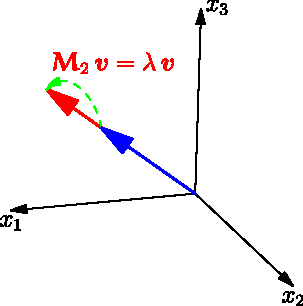
\includegraphics[width=0.4\linewidth]{eigenvector-2}
\end{center}
\keywords{Eigenvectors, Orthogonal Matrices, Eigenvector
  Decomposition, Rank}
%%%%%%%%%%%%%%%%%%%%%%% Next Slide %%%%%%%%%%%%%%%%%%%%%%%
\renewcommand{\Outline}{%
\begin{slide}
\section[1]{Outline}

\begin{minipage}{12cm}
  \begin{enumerate}\squeeze
    \outlineitem{Eigenvectors}{eigenvectors}
    \outlineitem{Orthogonal Matrices}{orthogonal}
    \outlineitem{Eigen Decomposition}{decomposition}
    \outlineitem{Low Rank Approximation}{lowrank}
    \outlineitem{Non-Normal Matrices}{nonnormal}
  \end{enumerate}
\end{minipage}\hfill
\begin{minipage}{10cm}
  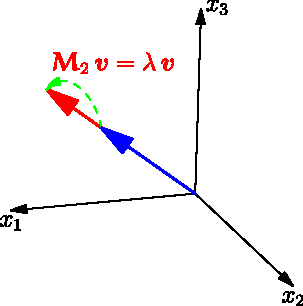
\includegraphics[height=10cm]{eigenvector-2}
\end{minipage}
\end{slide}
\addtocounter{outlineitem}{1}
}

\setcounter{outlineitem}{1}
\Outline % Eigenvectors
\toptarget{firstoutline}

%%%%%%%%%%%%%%%%%%%%%%% Next Slide %%%%%%%%%%%%%%%%%%%%%%%

\begin{slide}
\section[-2]{Eigenvector equation}
\pb

  \begin{itemize}
  \item Eigen-systems help us to understand mappings\pauseh
  \item A non-zero vector $\bm{v}$ is said to be an \emph{eigenvector} if
    \begin{minipage}{0.5\linewidth}
      \begin{displaymath}
        \mat{M} \bm{v} = \lambda \, \bm{v}\pauseh
      \end{displaymath}
    \end{minipage}\hfill
    \begin{minipage}{0.4\linewidth}
      \multipdf[height=7cm]{eigenvector}\pause
    \end{minipage}
  \item $\mat{M}$ is square (i.e. $n\stimes n$)\pauseh
  \item Where the number $\lambda$ is the \emph{eigenvalue}\pauseh
  \item Eigenvalues play a fundamental role in understanding operators\pauseh
  \end{itemize}


\end{slide}


%%%%%%%%%%%%%%%%%%%%%%% Next Slide %%%%%%%%%%%%%%%%%%%%%%%

\begin{slide}
\section[-1]{Symmetric Matrices}

\begin{PauseHighLight}
  \begin{itemize}
  \item If $\mat{M}$ is an $n\stimes n$ \emph{symmetric} matrix then it has
    $n$ real orthogonal eigenvectors with real eigenvalues\pause
  \item We denote the $i^{th}$ eigenvector by $\bm{v}_i$ and the
    corresponding eigenvalue by $\lambda_i$ so that
    \begin{displaymath}
      \mat{M} \bm{v}_i = \lambda_i \, \bm{v}_i \pause
    \end{displaymath}
  \item Orthogonal means that if $i\neq j$ then
    \begin{displaymath}
      \bm{v}_i^\tr \, \bm{v}_j = 0\pause
  \end{displaymath}
  \item (We can always normalise eigenvectors if we want)\pause
  \end{itemize}
\end{PauseHighLight}

\end{slide}


%%%%%%%%%%%%%%%%%%%%%%% Next Slide %%%%%%%%%%%%%%%%%%%%%%%

\begin{slide}
\section[-2]{Proof of Orthogonality}

\begin{PauseHighLight}
  \begin{itemize}
  \item $\left(\strut \mat{M}\bm{v}_i = \lambda_i\bm{v}_i\right)^\tr$
    implies $\bm{v}_i^\tr \mat{M}^\tr = \lambda_i\bm{v}_i^\tr$\pause
  \item When $\mat{M}$ is symmetric then $\mat{M}\bm{v}_i = \lambda_i\bm{v}_i
    \Rightarrow \bm{v}_i^\tr \mat{M} = \lambda_i\bm{v}_i^\tr$\pause
  \item Consider two eigenvectors $\bm{v}_i$ and $\bm{v}_j$ of $\mat{M}$
    \begin{align*}
      \bm{v}_i^\tr \mat{M} \bm{v}_j &= (\bm{v}_i^\tr \mat{M}) \bm{v}_j =
      \lambda_i  \bm{v}_i^\tr \bm{v}_j \\
      &= \bm{v}_i^\tr (\mat{M} \bm{v}_j)
      = \lambda_j  \bm{v}_i^\tr \bm{v}_j\pause
    \end{align*}
  \item So either $\lambda_i = \lambda_j$ or $\bm{v}_i^\tr \bm{v}_j=0$\pause
  \item If $\lambda_i = \lambda_j$ then any linear combination of
    $\bm{v}_i$ and $\bm{v}_j$ is an eigenvector
    ($\mat{M} (a\,\bm{v}_i + b\,\bm{v}_j) = \lambda_i (a\,\bm{v}_i +
    b\,\bm{v}_j) $)\pause.  So I can choose two eigenvectors that are
    orthogonal to each other.\pauseb
  \end{itemize}
\end{PauseHighLight}

\end{slide}

%%%%%%%%%%%%%%%%%%%%%%% Next Slide %%%%%%%%%%%%%%%%%%%%%%%
\Outline % Orthogonal Matrices
%%%%%%%%%%%%%%%%%%%%%%% Next Slide %%%%%%%%%%%%%%%%%%%%%%%

\begin{slide}
\section[-2]{Orthogonal Matrices}

\begin{PauseHighLight}
  \begin{itemize}
  \item We can construct an \emph{orthogonal} matrix $\mat{V}$ from the
    normalised eigenvectors ($\bm{v}_i^\tr\bm{v}_i = 1$)
    \begin{displaymath}
      \mat{V} = (\bm{v}_1, \bm{v}_2 , \cdots, \bm{v}_n)\pause
    \end{displaymath}
    \vspace*{-1cm}
  \item Matrix $\mat{V}$ is an $n\stimes n$ matrix\pause
  \item Because the vectors $\bm{v}_i$ are orthogonal and normalised
    \begin{displaymath}
      \mat{V}^\tr \, \mat{V} \pause =
      \begin{pmatrix}
        \bm{v}^\tr_1 \bm{v}_1 & \bm{v}^\tr_1 \bm{v}_2 & \cdots &
        \bm{v}^\tr_1 \bm{v}_n
        \\
        \bm{v}^\tr_2 \bm{v}_1 & \bm{v}^\tr_2 \bm{v}_2 & \cdots &
        \bm{v}^\tr_2 \bm{v}_n
        \\
        \vdots & \vdots & \ddots & \vdots
        \\
        \bm{v}^\tr_n \bm{v}_1 & \bm{v}^\tr_n \bm{v}_2 & \cdots &
        \bm{v}^\tr_n \bm{v}_n
      \end{pmatrix} \pause =
      \begin{pmatrix}
        1 & 0 & \cdots & 0 \\
        0 & 1 & \cdots & 0 \\
        \vdots & \vdots & \ddots & \vdots \\
        0 & 0 & \cdots & 1
      \end{pmatrix} \pause
      = \mat{I}\pause
    \end{displaymath}
  \end{itemize}
\end{PauseHighLight}

\end{slide}

%%%%%%%%%%%%%%%%%%%%%%% Next Slide %%%%%%%%%%%%%%%%%%%%%%%

\begin{slide}
\section[-2]{The Other Way Around}

\begin{PauseHighLight}
  \begin{itemize}
  \item We have shown that $\mat{V}^\tr \, \mat{V} = \mat{I}$\pause
  \item Thus multiply both sides on the left by $\mat{V}$
    \begin{align*}
      \mat{V}\,\mat{V}^\tr \, \mat{V} = \mat{V}\pause
    \end{align*}
  \item $\mat{V}$ will have an inverse (we show this on the next slide),
    $\mat{V}^{-1}$, such that
    $\mat{V} \, \mat{V}^{-1} = \mat{I}$\pause
  \item Multiplying the equation on the right by $\mat{V}^{-1}$
    \begin{align*}
      (\mat{V}\,\mat{V}^\tr) \, \mat{V} \, \mat{V}^{-1}
      &= \mat{V}\,\mat{V}^{-1}\pause  \\
      \mat{V}\,\mat{V}^\tr &= \mat{I}\pauseb
    \end{align*}
  \item Note that, $\mat{V}^{-1}=\mat{V}^\tr$ (definition of
    orthogonal matrix)\pause
  \end{itemize}
\end{PauseHighLight}

\end{slide}

%%%%%%%%%%%%%%%%%%%%%%% Next Slide %%%%%%%%%%%%%%%%%%%%%%%

\begin{slide}
\section[-2]{Invertible Matrices}

\begin{PauseHighLight}
  \begin{itemize}
  \item A matrix, $\mat{M}$, will be singular (not invertible) if there
    exists a vector $\bm{x}$ ($\neq\bm{0}$) such that
    \begin{align*}
      \mat{M}\,\bm{x} = \bm{0}\pause
    \end{align*}
  \item Now if there exists such a vector such that $\mat{V}\,\bm{x} =
    \bm{0}$ then multiplying by $\mat{V}^\tr$ we get
    \begin{align*}
      \mat{V}^\tr\, \mat{V}\, \bm{x} &= \mat{V}^\tr\, \bm{0} \pause \\
      \bm{x} &= \bm{0}
    \end{align*}
    since $\mat{V}^\tr\, \mat{V} = \mat{I}$\pauseb
  \item Thus $\mat{V}$ is invertible\pauseb
  \end{itemize}
\end{PauseHighLight}

\end{slide}



%%%%%%%%%%%%%%%%%%%%%%% Next Slide %%%%%%%%%%%%%%%%%%%%%%%

\begin{slide}
\section[-2]{Rotations}

\begin{PauseHighLight}
  \begin{itemize}
  \item Orthogonal matrices satisfy $\mat{V}^\tr \mat{V} = \mat{V}\,
    \mat{V}^\tr=\mat{I}$\pause
  \item As a consequence they define rotations (and possibly a reflection)\pause
  \item Consider a vector $\bm{x}$ and $\bm{x}'=\mat{V}\bm{x}$, now
    \begin{align*}
      \| \bm{x}' \|_2^2 = \bm{x}^{\prime\tr}\bm{x}'\pause
      = (\mat{V}\bm{x})^\tr (\mat{V}\bm{x})\pause
      = \bm{x}^\tr \mat{V}^\tr \mat{V} \bm{x}\pause
      = \bm{x}^\tr \bm{x} \pause = \| \bm{x} \|_2^2 \pause
    \end{align*}
  \item Similarly if additionally $\bm{y}'=\mat{V}\bm{y}$ then
    {\small
    \begin{align*}
      \langle \bm{x}', \bm{y}' \rangle = (\mat{V}\bm{x})^\tr
      (\mat{V}\bm{y})\pause
       = \bm{x}^\tr \mat{V}^\tr \mat{V} \bm{y}\pause
       = \bm{x}^\tr \bm{y} \pause = \langle \bm{x}, \bm{y} \rangle\pause
       = \| \bm{x} \|_2 \, \| \bm{y} \|_2 \, \cos(\theta)\pause
    \end{align*}}
  \item Rotations and reflections preserve lengths and angles\pause
  \end{itemize}
\end{PauseHighLight}

\end{slide}

%%%%%%%%%%%%%%%%%%%%%%% Next Slide %%%%%%%%%%%%%%%%%%%%%%%
\Outline % Matrix Decompostion
%%%%%%%%%%%%%%%%%%%%%%% Next Slide %%%%%%%%%%%%%%%%%%%%%%%

\begin{slide}
\section[-2]{Matrix Decomposition}

\begin{PauseHighLight}
  \begin{itemize}
  \item Taking the matrix of eigenvectors, $\mat{V}$, then
    \begin{align*}
      \mat{M}\, \mat{V}  &= \mat{M} (\bm{v}_1,\bm{v}_2,\ldots,\bm{v}_n)\pause
      =
      (\lambda_1\,\bm{v}_1,\lambda_2\,\bm{v}_2,\ldots,\lambda_n\,\bm{v}_n)\pause
      = \mat{V} \,\mat{\Lambda}
    \end{align*}
  \item where $\mat{\Lambda} = \mathrm{diag}(\lambda_1,
    \lambda_2,\ldots, \lambda_n) =
    \begin{pmatrix}
      \lambda_1 & 0 & \cdots & 0 \\
      0 & \lambda_2  & \cdots & 0 \\
      \vdots & \vdots &\ddots &\vdots \\
      0 & 0 & \cdots & \lambda_n
    \end{pmatrix}$\pause
  \item Now
    \begin{align*}
      \mat{M} = \mat{M}\, \mat{V} \, \mat{V}^\tr = \mat{V}
      \,\mat{\Lambda} \, \mat{V}^\tr \pause
    \end{align*}
  \item Very important \textit{similarity transform}\pause
  \end{itemize}
\end{PauseHighLight}

\end{slide}


%%%%%%%%%%%%%%%%%%%%%%% Next Slide %%%%%%%%%%%%%%%%%%%%%%%

\begin{slide}
\section[-2]{Mappings by Symmetric Matrices}

\pb \pause\pauselevel{=1}
\begin{center}
  \multipdf[width=\linewidth]{symmatrixPicture}\pause
\end{center}
\end{slide}


%%%%%%%%%%%%%%%%%%%%%%% Next Slide %%%%%%%%%%%%%%%%%%%%%%%

\begin{slide}
\section[-2]{Inverses}

\begin{PauseHighLight}
  \begin{itemize}
  \item For any symmetric invertible matrix
    \begin{align*}
      \mat{M} &=\mat{V}\,\mat{\Lambda}\,\mat{V}^\tr \pause &
      \mat{M}^{-1} &=\mat{V}\,\mat{\Lambda}^{-1}\,\mat{V}^\tr
    \end{align*}
  \item Where $\mat{\Lambda}^{-1} = \diag(\tfrac{1}{\lambda_1},
    \tfrac{1}{\lambda_2}, \ldots, \tfrac{1}{\lambda_n}) =
    \begin{pmatrix}
      \tfrac{1}{\lambda_1} & 0 & \cdots & 0 \\
      0 & \tfrac{1}{\lambda_2}  & \cdots & 0 \\
      \vdots & \vdots &\ddots &\vdots \\
      0 & 0 & \cdots & \tfrac{1}{\lambda_n}
    \end{pmatrix}$\pause
  \item Since
    \begin{align*}
       \mat{M}\,\mat{M}^{-1} &= (\mat{V}\,\mat{\Lambda}\,\mat{V}^\tr)\,
       (\mat{V}\,\mat{\Lambda}^{-1}\,\mat{V}^\tr)\pause
       = \mat{V}\,\mat{\Lambda}\,(\mat{V}^\tr\,
       \mat{V})\,\mat{\Lambda}^{-1}\,\mat{V}^\tr\pause \\
       &= \mat{V}\,\mat{\Lambda}\,\mat{\Lambda}^{-1}\,\mat{V}^\tr\pause
       = \mat{V}\,\mat{V}^\tr = \mat{I}\pause
    \end{align*}
  \item I.e.{} small eigenvalues become large eigenvalues and vice versa\pause
  \end{itemize}
\end{PauseHighLight}

\end{slide}

%%%%%%%%%%%%%%%%%%%%%%% Next Slide %%%%%%%%%%%%%%%%%%%%%%%

\begin{slide}
\section[-1.5]{Ill-Conditioning Again}

\pb\pause\pauselevel{=1}
\begin{center}
  \multipdf[width=0.9\linewidth]{conditioning}\pause
\end{center}

\end{slide}

%%%%%%%%%%%%%%%%%%%%%%% Next Slide %%%%%%%%%%%%%%%%%%%%%%%

\begin{slide}
\section[-2]{Condition Number}

\begin{PauseHighLight}
  \begin{itemize}\squeeze
  \item Taking matrix inverses can be inherently unstable\pause
  \item Any small error can be amplified by taking the inverse\pause
  \item The stability of the inverse depends on the ratio of smallest
    eigenvalue to the largest eigenvalue (i.e. the biggest possible
    amplification compared to the smallest)\pause
  \item For symmetric matrices the largest $|\lambda|$ is the spectral
    norm, $\|\mat{M}\|_2$, from the vector spaces lecture\pause
  \item The condition number is given by
    \begin{align*}
      \|\mat{M}\|_2 \times \|\mat{M}^{-1}\|_2 =
      \frac{|\lambda_{\text{\small max}}|}{|\lambda_{\text{\small min}}|}\pause
    \end{align*}
  \item Large condition number implies very ill-conditioned\pause
  \end{itemize}
\end{PauseHighLight}

\end{slide}

%%%%%%%%%%%%%%%%%%%%%%% Next Slide %%%%%%%%%%%%%%%%%%%%%%%
\Outline % Low Rank Approximation
%%%%%%%%%%%%%%%%%%%%%%% Next Slide %%%%%%%%%%%%%%%%%%%%%%%

\begin{slide}
\section[-1]{Rank of a Matrix}

\begin{PauseHighLight}
  \begin{itemize}
  \item The rank of a symmetric matrix, $\mat{M}$, is the number of non-zero
    eigenvalues\pause
  \item The space spanned by the eigenvectors $\bm{v}_a$, $\bm{v}_b$,
    etc.{} with zero eigenvalue forms a \emph{null space}\pause
  \item Any vector in the null space will get mapped to the zero
    vector
    \begin{align*}
      \mat{M} \, (a\, \bm{v}_a + b \, \bm{v}_b + \cdots) = \bm{0}\pause
    \end{align*}
  \item A square matrix is said to be \emph{rank deficient} if it has
    any eigenvectors with eigenvalue equal to 0\pause
   \item This happens when the columns of the matrix are not linearly independent\pause
 \end{itemize}
\end{PauseHighLight}

\end{slide}

%%%%%%%%%%%%%%%%%%%%%%% Next Slide %%%%%%%%%%%%%%%%%%%%%%%

\begin{slide}
\section[-2]{``Inverting'' Rank Deficient Matrices}

\begin{PauseHighLight}
  \begin{itemize}
  \item Rank deficient matrices are non-invertible (i.e. we don't know
    the vector $\bm{x}$ such that $\mat{M} \bm{x} = \bm{b}$) as we don't know
    the component of the $\bm{x}$ in the null space\pause
  \item Although we don't know $\bm{x}$ we can find a vector,
    $\bm{x}$, that satisfies $\mat{M} \bm{x} = \bm{b}$ (provided one
    exists)\pause
  \item Given a symmetric $n\times n$ matrix with $k$ non-zero eigenvalues
    $\lambda_1$, $\lambda_2$, $\ldots$, $\lambda_k$ we can construct
    a ``pseudo-inverse'' $\mat{M}^{+}$ as $\mat{V} \mat{\Lambda}^+
    \mat{V}^\tr$ where  $\mat{\Lambda}^{+} = \diag(\tfrac{1}{\lambda_1},
    \tfrac{1}{\lambda_2}, \ldots, \tfrac{1}{\lambda_k}, 0, \ldots,0)$\pause
  \item This finds the vector $\bm{x}$ with no component in the null
    space\pause{} (it is the solution with the smallest norm)\pauseb
  \item This and $(\mat{X}^\tr\mat{X})^{-1}\mat{X}^\tr$ are special
    cases of the pseudo-inverse we meet with SVD\pause
  \end{itemize}
\end{PauseHighLight}

\end{slide}

%%%%%%%%%%%%%%%%%%%%%%% Next Slide %%%%%%%%%%%%%%%%%%%%%%%

\begin{slide}
\section{Low Rank Approximation}

\begin{PauseHighLight}
  \begin{itemize}
  \item Recall that matrices with large and small eigenvalues are
    ill-conditioned so the inverse has the potential to greatly amplify any
    measurement error\pause
  \item One work around is to set all small eigenvalues to zero and
    use the pseudo-inverse\pause
  \item Setting small eigenvalues to zero reduces the rank of the
    matrix and is an example of a low rank approximation\pause
  \item Low rank approximations are much used to obtain approximate
    models for arrays of data\pause{} (we will revisit this when we look at SVD)\pauseb
  \end{itemize}
\end{PauseHighLight}

\end{slide}

%%%%%%%%%%%%%%%%%%%%%%% Next Slide %%%%%%%%%%%%%%%%%%%%%%%
\Outline % Non-Normal Matrices
%%%%%%%%%%%%%%%%%%%%%%% Next Slide %%%%%%%%%%%%%%%%%%%%%%%

\begin{slide}
\section[-2]{Non-Normal Matrices}

\begin{PauseHighLight}
  \begin{itemize}\squeeze
  \item Symmetric matrices are part of a class of matrices known as
    \emph{normal matrices}, which satisfy $\mat{M}\,\mat{M}^\dagger =
    \mat{M}^\dagger\mat{M}$\pause{} (for real matrices
    $\mat{M}^\dagger = \mat{M}^\tr$)\pauseb
  \item Hermitian matrices, $\mat{H}$, are complex matrices that equal
    their conjugate transpose: $\mat{H} = (\mat{H}^\tr)^*
    =\mat{H}^\dagger$\pause
  \item Hermitian matrices are also normal; they are important in
    quantum theory, less so in machine learning\pause
  \item Normal matrices are exactly those with a full set of orthonormal
    (possibly complex) eigenvectors\pause
  \item Most non-symmetric real matrices are not normal (rotations are
    an exception); their eigenvectors are more confusing\pause
  \end{itemize}
\end{PauseHighLight}

\end{slide}

%%%%%%%%%%%%%%%%%%%%%%% Next Slide %%%%%%%%%%%%%%%%%%%%%%%

\begin{slide}
\section[-2]{Asymmetric Matrices}

\begin{PauseHighLight}
  \begin{itemize}\squeeze
  \item For $n\times n$ real symmetric matrices we are guaranteed there are
    $n$ orthogonal real eigenvectors\pause
  \item For non-symmetric matrices the eigenvectors will generally not
    be orthogonal, they won't necessarily be real\pause
  \item We are not even guaranteed there will be $n$ linearly
    independent eigenvectors\pause
  \item Matrices which don't have $n$ linearly independent
    eigenvectors are said to be \emph{defective}, e.g.{}
    $\begin{pmatrix} 1 & 1 \\ 0 & 1 \end{pmatrix}$ has only one\pause
  \item Randomly generated matrices will typically not be defective,
    but nevertheless they can arise in certain situations\pause
  \end{itemize}
\end{PauseHighLight}

\end{slide}

%%%%%%%%%%%%%%%%%%%%%%% Next Slide %%%%%%%%%%%%%%%%%%%%%%%

\begin{slide}
\section{Characteristic Equation}

\begin{PauseHighLight}
  \begin{itemize}
  \item Since our eigenvectors are defined by  $\mat{M}\,\bm{v} =
    \lambda\,\bm{v}$ then
    \begin{align*}
      \bra{\strut \mat{M}-\lambda\mat{I}} \bm{v} &= \bm{0}
      & &\text{has a solution $\bm{v}\neq\bm{0}$ only if} &
      \det\bra{\strut \mat{M}-\lambda\mat{I}} = 0\pause
    \end{align*}
  \item This is known as the characteristic equation and leads to an
    $n^{th}$ order polynomial in $\lambda$\pause
  \item An $n^{th}$ order polynomial has $n$ roots (counting repeats),
    which are in general complex\pause
  \item Thus even for real (non-symmetric) matrices we can get complex
    eigenvalues\pause 
  \end{itemize}
\end{PauseHighLight}

\end{slide}

%%%%%%%%%%%%%%%%%%%%%%% Next Slide %%%%%%%%%%%%%%%%%%%%%%%

\begin{slide}
\section{Complex Conjugate Pairs}

\begin{PauseHighLight}
  \begin{itemize}
  \item If $\mat{M}$ is real and $\lambda$ is complex then $\bm{v}$ must
    be complex too, otherwise $\mat{M}\,\bm{v}$ would be real but
    $\lambda\,\bm{v}$ would not\pause
  \item Furthermore
    \begin{align*}
      \mat{M}\,\bm{v} &= \lambda\,\bm{v} & &\implies& \mat{M}\,\bm{v}^* &= \lambda^*\,\bm{v}^*\pause
    \end{align*}
  \item So that eigenvectors and their corresponding eigenvalues exist
    in complex conjugate pairs\pause
  \end{itemize}
\end{PauseHighLight}

\end{slide}

%%%%%%%%%%%%%%%%%%%%%%% Next Slide %%%%%%%%%%%%%%%%%%%%%%%

\begin{slide}
\section[-2]{Left and Right Eigenvectors}
  
\begin{PauseHighLight}\squeeze
  \begin{itemize}
  \item For symmetric matrices if $\bm{v}$ is a right-hand eigenvector
    in the sense that $\mat{M}\,\bm{v} = \lambda\, \bm{v}$ then
    $\bm{v}^\tr$ is a left-hand eigenvector
    \begin{align*}
      \bm{v}^\tr \mat{M} = \lambda\, \bm{v}^\tr\pause
    \end{align*}
  \item Earlier we used this property to show that the eigenvectors
    for symmetric matrices are orthogonal\pause
  \item For asymmetric real matrices the left-hand eigenvectors
    $\bm{u}^\tr$ are different from the right-hand eigenvectors, although
    they share the same eigenvalues (they have the same characteristic
    equation)
    \begin{align*}
      \mat{M}\,\bm{v} &= \lambda\, \bm{v}
      & \bm{u}^\tr\,\mat{M} = \lambda \, \bm{u}^\tr\pause
    \end{align*}
  \item As before, $\bm{u}_i^\tr\bm{v}_j = 0$ if
    $\lambda_i\neq\lambda_j$, but in general
    $\bm{v}_i^\tr\,\bm{v}_j\neq 0$\pause
  \end{itemize}
\end{PauseHighLight}

\end{slide}

%%%%%%%%%%%%%%%%%%%%%%% Next Slide %%%%%%%%%%%%%%%%%%%%%%%

\begin{slide}
\section{Eigen-Decomposition}

\begin{PauseHighLight}
  \begin{itemize}
  \item For a non-symmetric matrix, $\mat{M}$, provided it is
    not defective, we can decompose the matrix as
    \begin{align*}
      \mat{M} = \mat{V}\,\mat{\Lambda}\,\mat{V}^{-1}\pause
    \end{align*}
  \item $\mat{\Lambda}$ is a diagonal matrix of eigenvalues\pause
  \item $\mat{V}$ is a matrix whose columns are the right-hand
    eigenvectors\pause---in general it is not an orthogonal matrix\pauseb
  \item $\mat{V}^{-1}$ is a matrix whose rows are the left-hand
    eigenvectors\pause{} (scaled so that $\bm{u}_i^\tr\bm{v}_i = 1$)\pauseb
  \end{itemize}
\end{PauseHighLight}

\end{slide}


%%%%%%%%%%%%%%%%%%%%%%% Next Slide %%%%%%%%%%%%%%%%%%%%%%%

\begin{slide}
\section[-2]{Summary}

\begin{PauseHighLight}
  \begin{itemize}
  \item Linear mappings are commonly used in machine learning algorithms
    such as regression\pause
  \item We can understand symmetric operators by looking at their eigenvectors\pause
  \item Any symmetric matrix can be decomposed as $\mat{M} = \mat{V}
    \mat{\Lambda} \mat{V}^\tr$
    \begin{itemize}
    \item where $\mat{V}$ is an orthogonal matrix whose columns are the eigenvectors
    \item and $\mat{\Lambda}$ is a diagonal matrix of the eigenvalues\pause
    \end{itemize}
  \item This decomposition allows us to understand inverse
    mappings\pause
  \item Non-symmetric matrices are more complex\pause---we use the
    eigen-decomposition less because of this\pauseb
  \end{itemize}
\end{PauseHighLight}

\end{slide}


%%% Local Variables:
%%% TeX-master: "lectures"
%%% End:

\end{document}
